% !TEX root = ../Vorlage_DA.tex
%	########################################################
% 				Aufgabenstellung/Pflichtenheft
%	########################################################


%	--------------------------------------------------------
% 	Überschrift, Inhaltsverzeichnis
%	--------------------------------------------------------
\chapter{Einleitung}


%	--------------------------------------------------------
% 	Section 1
%	--------------------------------------------------------
\section{Einführung in sunnyHOME}
    
    Um im Urlaub zu sehen, wie das Wetter zurzeit zu Hause ist, musste man bisher immer bei öffentlichen Wetterberichten nachschauen. Diese sind jedoch nicht immer präzise. Das soll nun geändert werden, indem eine Hardware entwickelt werden wird, welche Wetterdaten sammelt und versendet.

    \begin{figure}[H]
        \centering
        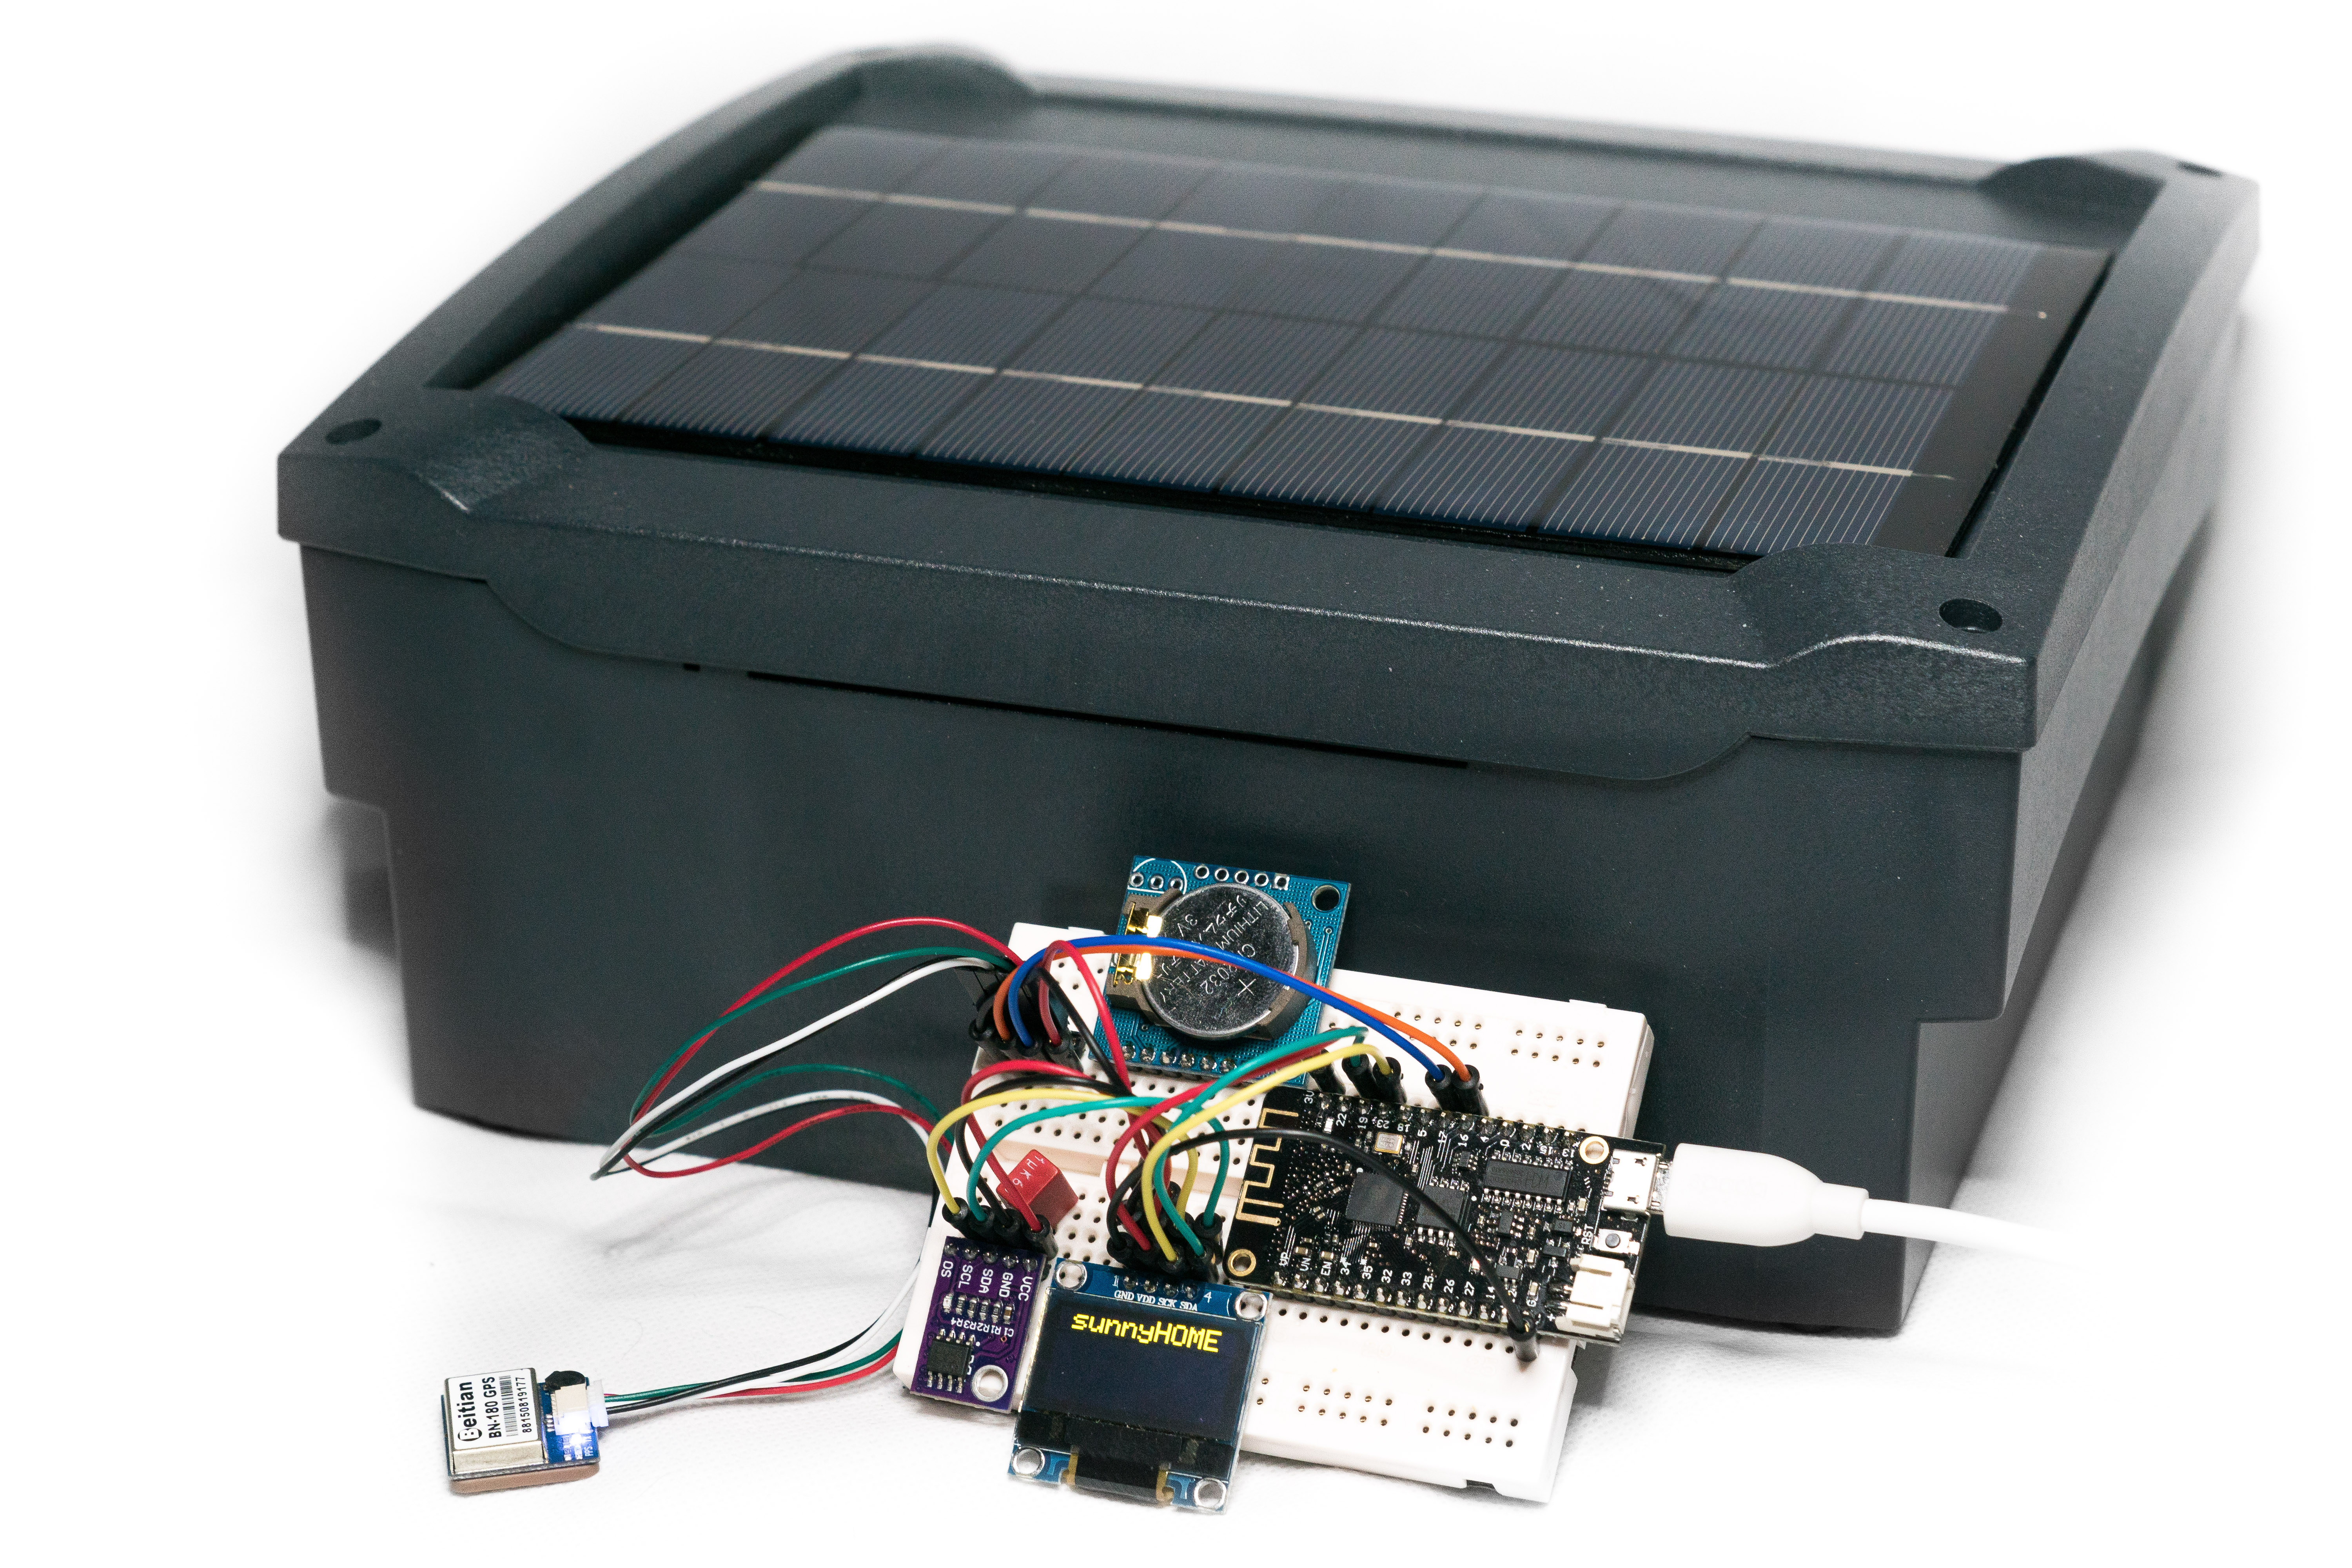
\includegraphics[width=0.7\textwidth]{./media/images/sunnyHOME.png}
        \caption{sunnyHOME-Logo}
        \label{fig:Logo}
    \end{figure}
    
    sunnyHOME ist ein Gerät, welches Wetterdaten sammelt und kabellos an einen Empfänger weiter sendet. 
    
    Es können verschiedene Sensoren, wie zum Beispiel Niederschlags- und UV-Sensoren verwendet werden. Die Daten der Sensoren werden dann über einen Mikrocontroller eingelesen und an einen Web-Server gesendet. Dieser wertet die Daten aus, die dann über eine Website oder eine App visualisiert werden. Somit kann man von überall auf der Welt nachschauen, ob die Blumen im Garten genug Wasser bekommen oder nicht.  

    
    

\pagebreak

%	--------------------------------------------------------
% 	Section 2:  Organisation
%	--------------------------------------------------------
\section{Organisation}
Das Projekt ``sunnyHOME'' wurde mit Hilfe von verschiedenen Tools organisiert. Die grundlegendsten sind in den folgenden Seiten beschrieben.
%\begin{description}

    \subsection{Microsoft To-Do}

        \begin{figure}[H]
            \centering
            \includegraphics[width=1\textwidth]{./media/images/TO-DO.png}
            \caption{Microsoft To-Do Screenshot}
            \label{fig:ToDo}
        \end{figure}
        
        \ \\ Microsoft To-Do ist eine übliche To-Do-Listen Applikation. Sie ist für Windows, Android sowie iOS verfügbar. Man kann zwischen Aufgabenbereichen trennen, und den einzelnen Aufgaben Termine zuweisen. Erstellte Termine werden über das Microsoft-Konto synchronisiert, und um einen guten Überblick über die kommende Agenda zu haben, im Kalender angezeigt.

\pagebreak
        
    \subsection{Excel}\label{ref:Protokoll}
    
        \ \\ Mit Hilfe von Microsoft Excel, sind die Arbeitszeiten und die durchgeführten Arbeitsschritte protokolliert worden. Man kann angeben, zu wie viel Prozent ein Arbeitsschritt fertiggestellt worden ist und ebenfalls Beschreibungen hinzufügen, was genau durchgeführt worden ist, wo sich Probleme ergeben haben, und was das nächste Mal gemacht werden sollte.
    
        \begin{figure}[H]
            \centering
            \includegraphics[width=1\textwidth]{./media/images/Excel.jpg}
            \caption{Protokoll Screenshot}
            \label{fig:Protokoll}
        \end{figure}
        
        Gerade bei größeren Projekten ist es sehr wichtig, Arbeitsschritte aus der Vergangenheit zurückverfolgen zu können. Sobald eine Woche nicht mehr gearbeitet wird, sind oft wichtige Ziele oder nicht vervollständigte Schritte vergessen. 
        
\pagebreak
        
        \subsubsection{Zeitplan}
        \begin{figure}[H]
            \centering
            \includegraphics[width=1\textwidth]{./media/images/Zeitplan.jpg}
            \caption{Zeitplan Screenshot}
            \label{fig:Zeitplan}
        \end{figure}
        
        Der in Excel erstellte Zeitplan ist quasi das Gegenstück zum Protokoll (siehe: \ref{ref:Protokoll}). Er visualisiert einem die kommenden Termine, und welche Arbeitsschritte in welcher Woche zu erledigen sind. Der Plan ist in Kalenderwochen strukturiert, wobei nur Arbeitstage gezählt werden. Außerdem werden einem zu beachtende Termine, Feiertage und Events neben den einzelnen Wochen angezeigt.
        
\pagebreak
        
        \subsubsection{Objektstrukturplan}\label{ref:Objektstrukt}
        
        Ebenfalls in Excel wurde ein Objektstrukturplan erstellt. Dieser orientiert sich an Projektergebnissen. Diese Projektergebnisse werden dann in Teilergebnisse aufgeteilt und hierarchisch untereinander gegliedert. 
        
        \begin{figure}[H]
            \centering
            \includegraphics[width=1\textwidth]{./media/images/Objektstrukturplan.jpg}
            \caption{Objektstrukturplan Screenshot}
            \label{fig:Objektstrukt}
        \end{figure}
        
        Vervollständigt wird der Objektstrukturplan durch einen Projektstrukturplan. (siehe \ref{ref:Projektstrukt})
        \begin{flushright}
            \cite{bib:Strukturpl}
        \end{flushright}
        
\pagebreak
        
        \subsubsection{Projektstrukturplan}\label{ref:Projektstrukt}
        
        Ein Projektstrukturplan orientiert sich hingegen einem Objektstrukturplan (siehe: \ref{ref:Objektstrukt}) nicht am Ergebnis, sondern an den Projektphasen. Es ist direkt bemerkbar, dass dieser detaillierter ist als der Objektstrukturplan. 
        
        \begin{figure}[H]
            \centering
            \includegraphics[width=1\textwidth]{./media/images/Projektstrukturplan.jpg}
            \caption{Projektstrukturplan Screenshot}
            \label{fig:Projektstrukt}
        \end{figure}
        
        
        Die Projektphasen werden von links nach rechts ihrer Durchführungsreihenfolge angeordnet. Lediglich das Projektmanagement bleibt immer links (siehe \ref{fig:Projektstrukt}: 1), da es von Anfang bis Ende des Projektes gemacht wird. Schlussendlich endet jede Arbeitsphase mit einem Meilenstein, der das Ende der Phase kennzeichnet. 
        
        \begin{flushright}
            \cite{bib:Strukturpl}
        \end{flushright}
        
        
        
\pagebreak

    \subsection{GitHub}\label{ref:GitHub}
        \ \\ Ein großer Teil des Projektmanagements ist über GitHub gelaufen. Mit Hilfe von GitHub können andere Menschen einen kompletten Überblick über das Projekt erhalten. Dafür gibt es eine Main-Page, über welche man das Datei-Verzeichnis ansehen und eine Zusammenfassung des Projektes lesen kann. Quellcodes sind für jeden zugänglich, und sogar vergangene Veränderungen an diesen sind anschaubar. Zudem ist es möglich, ein projekteigenes Wiki zu erstellen. GitHub wurde in diesem Projekt aber hauptsächlich wegen der Online-Synchronisierung verwendet. Um die Synchronisierung leichter zu gestalten, gibt es eine Desktopanwendung, welche Veränderungen hochlädt und neuste Updates herunterlädt. Dadurch lässt es sich von jedem beliebigen PC, am Projekt weiterarbeiten. 
        
        \begin{figure}[H]
            \centering
            \includegraphics[width=0.8\textwidth]{./media/images/GitHub.jpg}
            \caption{GitHub Screenshot}
            \label{fig:GitHub}
        \end{figure}
        
\pagebreak
        
    \subsection{Microsoft Project} \label{ref:MSProject}
    
        \begin{figure}[H]
            \centering
            \includegraphics[width=1\textwidth]{./media/images/GANTT.jpg}
            \caption{Mit Microsoft Project erstelltes GANTT-Diagramm}
            \label{fig:GANTT}
        \end{figure}
        
        \ \\ Mit Microsoft Project lassen sich spielend leicht, komplexe GANTT-Diagramme erstellen. Das Diagramm macht es dann möglich, dem Betrachter einen guten Rundumblick über das gegebene Projekt zu bieten. Vor allem für Außenstehende, welche sich über das Projekt und dessen Fortschritt informieren wollen, eignet es sich hervorragend. Man sieht, wann welche Arbeitsschritte durchgeführt wurden, was zurzeit das Thema ist, und welcher Arbeitsschritt der Zukunft, zu welchem Zeitpunkt ansteht. Die angegebenen Arbeitsschritte sind hierbei die selben, welche auch im Projektstrukturplan zu finden sind (siehe \ref{ref:Projektstrukt}).
%\end{description}

\pagebreak

%	--------------------------------------------------------
% 	Section 3:  Zielsetzung
%	--------------------------------------------------------
\section{Zielsetzung}
    Es soll eine Hardware entwickelt werden, die verschiedene Wetterdaten vor Ort sammelt, und über einen Web-Server von überall abgreifbar macht. Ein weiteres Ziel ist es Mithilfe von Website und App Daten übersichtlich zu visualisieren.
    
    \underline{\textbf{Die wichtigsten 5 Meilensteine: }}
    \begin{itemize}
        \item Konzept fertig
        \item Hardware funktioniert
        \item Software funktioniert
        \item Datenübertragung funktioniert 
        \item Diplomarbeit verfasst 
    \end{itemize}
    
    \subsection{Prioritäten}
    Zum einen sollte die Wetterstation sich selbst mit Energie versorgen können. Dann sollte sie modular sein, damit Hobby-Bastler leicht zwischen Funktionalitäten wechseln können. Aus diesem Grund ist das Projekt auch Open-Source (siehe: \ref{ref:GitHub}). Es soll eine grafische Benutzeroberfläche entstehen, von der aus man alles gut im Blick hat. Die Box soll dann zusätzlich über GPS lokalisiert werden können.
    Die folgenden Meilensteine sind nach Priorität sortiert.
    
    \begin{enumerate}
        \item Ein Energie-effizientes System welches Unabhängig von einer Stromversorgung ist
        \item Ein System zur Übertragung der Daten welches Energie-effizient ist
        \item Eine Hardware die multifunktional mit verschiedenen Sensoren kompatibel ist
        \item Ein einfaches modulares System, um beliebige Sensoren anzubringen 
        \item Energie-effiziente Sensoren
    \end{enumerate}
